\documentclass[1p]{elsarticle_modified}
%\bibliographystyle{elsarticle-num}

%\usepackage[colorlinks]{hyperref}
%\usepackage{abbrmath_seonhwa} %\Abb, \Ascr, \Acal ,\Abf, \Afrak
\usepackage{amsfonts}
\usepackage{amssymb}
\usepackage{amsmath}
\usepackage{amsthm}
\usepackage{scalefnt}
\usepackage{amsbsy}
\usepackage{kotex}
\usepackage{caption}
\usepackage{subfig}
\usepackage{color}
\usepackage{graphicx}
\usepackage{xcolor} %% white, black, red, green, blue, cyan, magenta, yellow
\usepackage{float}
\usepackage{setspace}
\usepackage{hyperref}

\usepackage{tikz}
\usetikzlibrary{arrows}

\usepackage{multirow}
\usepackage{array} % fixed length table
\usepackage{hhline}

%%%%%%%%%%%%%%%%%%%%%
\makeatletter
\renewcommand*\env@matrix[1][\arraystretch]{%
	\edef\arraystretch{#1}%
	\hskip -\arraycolsep
	\let\@ifnextchar\new@ifnextchar
	\array{*\c@MaxMatrixCols c}}
\makeatother %https://tex.stackexchange.com/questions/14071/how-can-i-increase-the-line-spacing-in-a-matrix
%%%%%%%%%%%%%%%

\usepackage[normalem]{ulem}

\newcommand{\msout}[1]{\ifmmode\text{\sout{\ensuremath{#1}}}\else\sout{#1}\fi}
%SOURCE: \msout is \stkout macro in https://tex.stackexchange.com/questions/20609/strikeout-in-math-mode

\newcommand{\cancel}[1]{
	\ifmmode
	{\color{red}\msout{#1}}
	\else
	{\color{red}\sout{#1}}
	\fi
}

\newcommand{\add}[1]{
	{\color{blue}\uwave{#1}}
}

\newcommand{\replace}[2]{
	\ifmmode
	{\color{red}\msout{#1}}{\color{blue}\uwave{#2}}
	\else
	{\color{red}\sout{#1}}{\color{blue}\uwave{#2}}
	\fi
}

\newcommand{\Sol}{\mathcal{S}} %segment
\newcommand{\D}{D} %diagram
\newcommand{\A}{\mathcal{A}} %arc


%%%%%%%%%%%%%%%%%%%%%%%%%%%%%5 test

\def\sl{\operatorname{\textup{SL}}(2,\Cbb)}
\def\psl{\operatorname{\textup{PSL}}(2,\Cbb)}
\def\quan{\mkern 1mu \triangleright \mkern 1mu}

\theoremstyle{definition}
\newtheorem{thm}{Theorem}[section]
\newtheorem{prop}[thm]{Proposition}
\newtheorem{lem}[thm]{Lemma}
\newtheorem{ques}[thm]{Question}
\newtheorem{cor}[thm]{Corollary}
\newtheorem{defn}[thm]{Definition}
\newtheorem{exam}[thm]{Example}
\newtheorem{rmk}[thm]{Remark}
\newtheorem{alg}[thm]{Algorithm}

\newcommand{\I}{\sqrt{-1}}
\begin{document}

%\begin{frontmatter}
%
%\title{Boundary parabolic representations of knots up to 8 crossings}
%
%%% Group authors per affiliation:
%\author{Yunhi Cho} 
%\address{Department of Mathematics, University of Seoul, Seoul, Korea}
%\ead{yhcho@uos.ac.kr}
%
%
%\author{Seonhwa Kim} %\fnref{s_kim}}
%\address{Center for Geometry and Physics, Institute for Basic Science, Pohang, 37673, Korea}
%\ead{ryeona17@ibs.re.kr}
%
%\author{Hyuk Kim}
%\address{Department of Mathematical Sciences, Seoul National University, Seoul 08826, Korea}
%\ead{hyukkim@snu.ac.kr}
%
%\author{Seokbeom Yoon}
%\address{Department of Mathematical Sciences, Seoul National University, Seoul, 08826,  Korea}
%\ead{sbyoon15@snu.ac.kr}
%
%\begin{abstract}
%We find all boundary parabolic representation of knots up to 8 crossings.
%
%\end{abstract}
%\begin{keyword}
%    \MSC[2010] 57M25 
%\end{keyword}
%
%\end{frontmatter}

%\linenumbers
%\tableofcontents
%
\newcommand\colored[1]{\textcolor{white}{\rule[-0.35ex]{0.8em}{1.4ex}}\kern-0.8em\color{red} #1}%
%\newcommand\colored[1]{\textcolor{white}{ #1}\kern-2.17ex	\textcolor{white}{ #1}\kern-1.81ex	\textcolor{white}{ #1}\kern-2.15ex\color{red}#1	}

{\Large $\underline{12a_{0185}~(K12a_{0185})}$}

\setlength{\tabcolsep}{10pt}
\renewcommand{\arraystretch}{1.6}
\vspace{1cm}\begin{tabular}{m{100pt}>{\centering\arraybackslash}m{274pt}}
\multirow{5}{120pt}{
	\centering
	\includegraphics[width=112pt]{../../../GIT/diagram.site/Diagrams/png/986_12a_0185.png}\\
\ \ \ A knot diagram\footnotemark}&
\allowdisplaybreaks
\textbf{Linearized knot diagam} \\
\cline{2-2}
 &
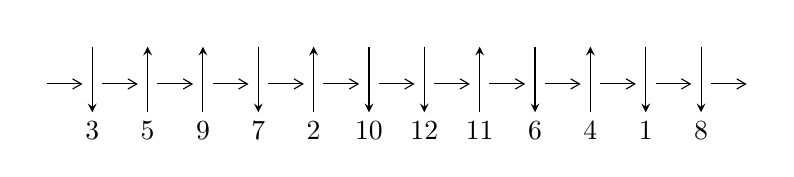
\begin{tikzpicture}[x=20pt, y=17pt]
	% nodes
	\node (C0) at (0, 0) {};
	\node (C1) at (1, 0) {};
	\node (C1U) at (1, +1) {};
	\node (C1D) at (1, -1) {3};

	\node (C2) at (2, 0) {};
	\node (C2U) at (2, +1) {};
	\node (C2D) at (2, -1) {5};

	\node (C3) at (3, 0) {};
	\node (C3U) at (3, +1) {};
	\node (C3D) at (3, -1) {9};

	\node (C4) at (4, 0) {};
	\node (C4U) at (4, +1) {};
	\node (C4D) at (4, -1) {7};

	\node (C5) at (5, 0) {};
	\node (C5U) at (5, +1) {};
	\node (C5D) at (5, -1) {2};

	\node (C6) at (6, 0) {};
	\node (C6U) at (6, +1) {};
	\node (C6D) at (6, -1) {10};

	\node (C7) at (7, 0) {};
	\node (C7U) at (7, +1) {};
	\node (C7D) at (7, -1) {12};

	\node (C8) at (8, 0) {};
	\node (C8U) at (8, +1) {};
	\node (C8D) at (8, -1) {11};

	\node (C9) at (9, 0) {};
	\node (C9U) at (9, +1) {};
	\node (C9D) at (9, -1) {6};

	\node (C10) at (10, 0) {};
	\node (C10U) at (10, +1) {};
	\node (C10D) at (10, -1) {4};

	\node (C11) at (11, 0) {};
	\node (C11U) at (11, +1) {};
	\node (C11D) at (11, -1) {1};

	\node (C12) at (12, 0) {};
	\node (C12U) at (12, +1) {};
	\node (C12D) at (12, -1) {8};
	\node (C13) at (13, 0) {};

	% arrows
	\draw[->,>={angle 60}]
	(C0) edge (C1) (C1) edge (C2) (C2) edge (C3) (C3) edge (C4) (C4) edge (C5) (C5) edge (C6) (C6) edge (C7) (C7) edge (C8) (C8) edge (C9) (C9) edge (C10) (C10) edge (C11) (C11) edge (C12) (C12) edge (C13) ;	\draw[->,>=stealth]
	(C1U) edge (C1D) (C2D) edge (C2U) (C3D) edge (C3U) (C4U) edge (C4D) (C5D) edge (C5U) (C6U) edge (C6D) (C7U) edge (C7D) (C8D) edge (C8U) (C9U) edge (C9D) (C10D) edge (C10U) (C11U) edge (C11D) (C12U) edge (C12D) ;
	\end{tikzpicture} \\
\hhline{~~} \\& 
\textbf{Solving Sequence} \\ \cline{2-2} 
 &
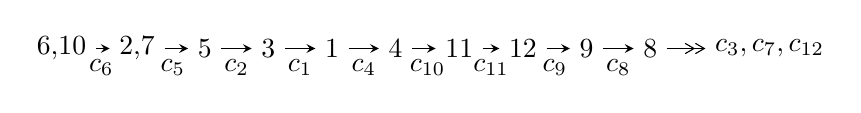
\begin{tikzpicture}[x=23pt, y=7pt]
	% node
	\node (A0) at (-1/8, 0) {6,10};
	\node (A1) at (17/16, 0) {2,7};
	\node (A2) at (17/8, 0) {5};
	\node (A3) at (25/8, 0) {3};
	\node (A4) at (33/8, 0) {1};
	\node (A5) at (41/8, 0) {4};
	\node (A6) at (49/8, 0) {11};
	\node (A7) at (57/8, 0) {12};
	\node (A8) at (65/8, 0) {9};
	\node (A9) at (73/8, 0) {8};
	\node (C1) at (1/2, -1) {$c_{6}$};
	\node (C2) at (13/8, -1) {$c_{5}$};
	\node (C3) at (21/8, -1) {$c_{2}$};
	\node (C4) at (29/8, -1) {$c_{1}$};
	\node (C5) at (37/8, -1) {$c_{4}$};
	\node (C6) at (45/8, -1) {$c_{10}$};
	\node (C7) at (53/8, -1) {$c_{11}$};
	\node (C8) at (61/8, -1) {$c_{9}$};
	\node (C9) at (69/8, -1) {$c_{8}$};
	\node (A10) at (11, 0) {$c_{3},c_{7},c_{12}$};

	% edge
	\draw[->,>=stealth]	
	(A0) edge (A1) (A1) edge (A2) (A2) edge (A3) (A3) edge (A4) (A4) edge (A5) (A5) edge (A6) (A6) edge (A7) (A7) edge (A8) (A8) edge (A9) ;
	\draw[->>,>={angle 60}]	
	(A9) edge (A10);
\end{tikzpicture} \\ 

\end{tabular} \\

\footnotetext{
The image of knot diagram is generated by the software ``\textbf{Draw programme}" developed by Andrew Bartholomew(\url{http://www.layer8.co.uk/maths/draw/index.htm\#Running-draw}), where we modified some parts for our purpose(\url{https://github.com/CATsTAILs/LinksPainter}).
}\phantom \\ \newline 
\centering \textbf{Ideals for irreducible components\footnotemark of $X_{\text{par}}$} 
 
\begin{align*}
I^u_{1}&=\langle 
4.98914\times10^{445} u^{128}-1.30336\times10^{446} u^{127}+\cdots+2.09279\times10^{445} b+7.62318\times10^{445},\\
\phantom{I^u_{1}}&\phantom{= \langle  }5.11649\times10^{446} u^{128}-1.01386\times10^{447} u^{127}+\cdots+1.04639\times10^{446} a+3.19751\times10^{446},\;u^{129}-3 u^{128}+\cdots+6 u-1\rangle \\
I^u_{2}&=\langle 
2 u^2 a- a u+2 u^2+b+2 a- u+2,\;15 u^2 a+25 a^2-5 a u+13 u^2+60 a-6 u+42,\;u^3- u^2+2 u-1\rangle \\
\\
\end{align*}
\raggedright * 2 irreducible components of $\dim_{\mathbb{C}}=0$, with total 135 representations.\\
\footnotetext{All coefficients of polynomials are rational numbers. But the coefficients are sometimes approximated in decimal forms when there is not enough margin.}
\newpage
\renewcommand{\arraystretch}{1}
\centering \section*{I. $I^u_{1}= \langle 4.99\times10^{445} u^{128}-1.30\times10^{446} u^{127}+\cdots+2.09\times10^{445} b+7.62\times10^{445},\;5.12\times10^{446} u^{128}-1.01\times10^{447} u^{127}+\cdots+1.05\times10^{446} a+3.20\times10^{446},\;u^{129}-3 u^{128}+\cdots+6 u-1 \rangle$}
\flushleft \textbf{(i) Arc colorings}\\
\begin{tabular}{m{7pt} m{180pt} m{7pt} m{180pt} }
\flushright $a_{6}=$&$\begin{pmatrix}1\\0\end{pmatrix}$ \\
\flushright $a_{10}=$&$\begin{pmatrix}0\\u\end{pmatrix}$ \\
\flushright $a_{2}=$&$\begin{pmatrix}-4.88965 u^{128}+9.68913 u^{127}+\cdots+21.8288 u-3.05575\\-2.38397 u^{128}+6.22785 u^{127}+\cdots+17.3934 u-3.64260\end{pmatrix}$ \\
\flushright $a_{7}=$&$\begin{pmatrix}1\\u^2\end{pmatrix}$ \\
\flushright $a_{5}=$&$\begin{pmatrix}-16.2649 u^{128}+36.0614 u^{127}+\cdots+94.5515 u-18.4908\\4.05033 u^{128}-8.11181 u^{127}+\cdots-22.0327 u+3.82688\end{pmatrix}$ \\
\flushright $a_{3}=$&$\begin{pmatrix}-12.5725 u^{128}+28.3938 u^{127}+\cdots+72.9033 u-14.6140\\3.00818 u^{128}-5.66495 u^{127}+\cdots-14.4581 u+2.25274\end{pmatrix}$ \\
\flushright $a_{1}=$&$\begin{pmatrix}7.59367 u^{128}-17.3064 u^{127}+\cdots-46.4404 u+9.36540\\-0.489938 u^{128}+1.20604 u^{127}+\cdots+5.09923 u-1.11099\end{pmatrix}$ \\
\flushright $a_{4}=$&$\begin{pmatrix}-2.55440 u^{128}+6.03912 u^{127}+\cdots+12.3850 u-1.93084\\13.0262 u^{128}-28.0196 u^{127}+\cdots-74.9764 u+14.9359\end{pmatrix}$ \\
\flushright $a_{11}=$&$\begin{pmatrix}-1.11099 u^{128}+2.84302 u^{127}+\cdots+7.35949 u-1.56670\\5.47464 u^{128}-12.7709 u^{127}+\cdots-36.1966 u+7.59367\end{pmatrix}$ \\
\flushright $a_{12}=$&$\begin{pmatrix}-2.33366 u^{128}+5.14492 u^{127}+\cdots+17.3240 u-3.56421\\6.20152 u^{128}-15.0253 u^{127}+\cdots-43.6088 u+8.95686\end{pmatrix}$ \\
\flushright $a_{9}=$&$\begin{pmatrix}u\\u\end{pmatrix}$ \\
\flushright $a_{8}=$&$\begin{pmatrix}-3.44229 u^{128}+8.53517 u^{127}+\cdots+30.9440 u-5.97392\\4.25086 u^{128}-8.79384 u^{127}+\cdots-19.2212 u+3.91476\end{pmatrix}$\\&\end{tabular}
\flushleft \textbf{(ii) Obstruction class $= -1$}\\~\\
\flushleft \textbf{(iii) Cusp Shapes $= -35.3681 u^{128}+84.1056 u^{127}+\cdots+260.905 u-58.9553$}\\~\\
\newpage\renewcommand{\arraystretch}{1}
\flushleft \textbf{(iv) u-Polynomials at the component}\newline \\
\begin{tabular}{m{50pt}|m{274pt}}
Crossings & \hspace{64pt}u-Polynomials at each crossing \\
\hline $$\begin{aligned}c_{1}\end{aligned}$$&$\begin{aligned}
&u^{129}+58 u^{128}+\cdots+31691 u-625
\end{aligned}$\\
\hline $$\begin{aligned}c_{2},c_{5}\end{aligned}$$&$\begin{aligned}
&u^{129}+4 u^{128}+\cdots-129 u-25
\end{aligned}$\\
\hline $$\begin{aligned}c_{3}\end{aligned}$$&$\begin{aligned}
&25(25 u^{129}-195 u^{128}+\cdots+2.03112\times10^{7} u+1405871)
\end{aligned}$\\
\hline $$\begin{aligned}c_{4}\end{aligned}$$&$\begin{aligned}
&25(25 u^{129}-30 u^{128}+\cdots-2354708 u+76193)
\end{aligned}$\\
\hline $$\begin{aligned}c_{6},c_{9}\end{aligned}$$&$\begin{aligned}
&u^{129}+3 u^{128}+\cdots+6 u+1
\end{aligned}$\\
\hline $$\begin{aligned}c_{7},c_{12}\end{aligned}$$&$\begin{aligned}
&u^{129}+3 u^{128}+\cdots+2 u+1
\end{aligned}$\\
\hline $$\begin{aligned}c_{8}\end{aligned}$$&$\begin{aligned}
&u^{129}+9 u^{128}+\cdots+4123464 u+328729
\end{aligned}$\\
\hline $$\begin{aligned}c_{10}\end{aligned}$$&$\begin{aligned}
&u^{129}-3 u^{128}+\cdots+26400 u+8000
\end{aligned}$\\
\hline $$\begin{aligned}c_{11}\end{aligned}$$&$\begin{aligned}
&u^{129}+63 u^{128}+\cdots+6 u+1
\end{aligned}$\\
\hline
\end{tabular}\\~\\
\newpage\renewcommand{\arraystretch}{1}
\flushleft \textbf{(v) Riley Polynomials at the component}\newline \\
\begin{tabular}{m{50pt}|m{274pt}}
Crossings & \hspace{64pt}Riley Polynomials at each crossing \\
\hline $$\begin{aligned}c_{1}\end{aligned}$$&$\begin{aligned}
&y^{129}+30 y^{128}+\cdots+1330940731 y-390625
\end{aligned}$\\
\hline $$\begin{aligned}c_{2},c_{5}\end{aligned}$$&$\begin{aligned}
&y^{129}+58 y^{128}+\cdots+31691 y-625
\end{aligned}$\\
\hline $$\begin{aligned}c_{3}\end{aligned}$$&$\begin{aligned}
&625\\
&\cdot(625 y^{129}+26325 y^{128}+\cdots+27395194733737 y-1976473268641)
\end{aligned}$\\
\hline $$\begin{aligned}c_{4}\end{aligned}$$&$\begin{aligned}
&625(625 y^{129}-14300 y^{128}+\cdots+3.74977\times10^{11} y-5.80537\times10^{9})
\end{aligned}$\\
\hline $$\begin{aligned}c_{6},c_{9}\end{aligned}$$&$\begin{aligned}
&y^{129}-71 y^{128}+\cdots+6 y-1
\end{aligned}$\\
\hline $$\begin{aligned}c_{7},c_{12}\end{aligned}$$&$\begin{aligned}
&y^{129}-63 y^{128}+\cdots+6 y-1
\end{aligned}$\\
\hline $$\begin{aligned}c_{8}\end{aligned}$$&$\begin{aligned}
&y^{129}+45 y^{128}+\cdots+5854253992682 y-108062755441
\end{aligned}$\\
\hline $$\begin{aligned}c_{10}\end{aligned}$$&$\begin{aligned}
&y^{129}+35 y^{128}+\cdots-255360000 y-64000000
\end{aligned}$\\
\hline $$\begin{aligned}c_{11}\end{aligned}$$&$\begin{aligned}
&y^{129}+9 y^{128}+\cdots-14 y-1
\end{aligned}$\\
\hline
\end{tabular}\\~\\
\newpage\flushleft \textbf{(vi) Complex Volumes and Cusp Shapes}
$$\begin{array}{c|c|c}  
\text{Solutions to }I^u_{1}& \I (\text{vol} + \sqrt{-1}CS) & \text{Cusp shape}\\
 \hline 
\begin{aligned}
u &= -0.983463 + 0.268681 I \\
a &= -0.62036 + 1.96394 I \\
b &= \phantom{-}0.682768 + 1.129540 I\end{aligned}
 & -0.58814 + 4.93859 I & \phantom{-0.000000 } 0 \\ \hline\begin{aligned}
u &= -0.983463 - 0.268681 I \\
a &= -0.62036 - 1.96394 I \\
b &= \phantom{-}0.682768 - 1.129540 I\end{aligned}
 & -0.58814 - 4.93859 I & \phantom{-0.000000 } 0 \\ \hline\begin{aligned}
u &= -0.175616 + 0.948969 I \\
a &= \phantom{-}0.687811 - 0.298549 I \\
b &= -0.739891 - 0.477913 I\end{aligned}
 & \phantom{-}2.15356 - 3.17502 I & \phantom{-0.000000 } 0 \\ \hline\begin{aligned}
u &= -0.175616 - 0.948969 I \\
a &= \phantom{-}0.687811 + 0.298549 I \\
b &= -0.739891 + 0.477913 I\end{aligned}
 & \phantom{-}2.15356 + 3.17502 I & \phantom{-0.000000 } 0 \\ \hline\begin{aligned}
u &= \phantom{-}0.144632 + 0.952589 I \\
a &= \phantom{-}0.648121 + 0.279122 I \\
b &= -0.803079 + 0.453732 I\end{aligned}
 & -0.32991 + 8.26485 I & \phantom{-0.000000 } 0 \\ \hline\begin{aligned}
u &= \phantom{-}0.144632 - 0.952589 I \\
a &= \phantom{-}0.648121 - 0.279122 I \\
b &= -0.803079 - 0.453732 I\end{aligned}
 & -0.32991 - 8.26485 I & \phantom{-0.000000 } 0 \\ \hline\begin{aligned}
u &= \phantom{-}0.917821 + 0.279541 I \\
a &= -0.44055 - 1.58384 I \\
b &= \phantom{-}0.817754 - 1.027710 I\end{aligned}
 & -1.80994 - 1.27988 I & \phantom{-0.000000 } 0 \\ \hline\begin{aligned}
u &= \phantom{-}0.917821 - 0.279541 I \\
a &= -0.44055 + 1.58384 I \\
b &= \phantom{-}0.817754 + 1.027710 I\end{aligned}
 & -1.80994 + 1.27988 I & \phantom{-0.000000 } 0 \\ \hline\begin{aligned}
u &= -0.930509 + 0.131444 I \\
a &= \phantom{-}3.26267 + 1.98840 I \\
b &= \phantom{-}0.424467 - 0.884741 I\end{aligned}
 & -4.38795 - 5.53131 I & \phantom{-0.000000 } 0 \\ \hline\begin{aligned}
u &= -0.930509 - 0.131444 I \\
a &= \phantom{-}3.26267 - 1.98840 I \\
b &= \phantom{-}0.424467 + 0.884741 I\end{aligned}
 & -4.38795 + 5.53131 I & \phantom{-0.000000 } 0\\
 \hline 
 \end{array}$$\newpage$$\begin{array}{c|c|c}  
\text{Solutions to }I^u_{1}& \I (\text{vol} + \sqrt{-1}CS) & \text{Cusp shape}\\
 \hline 
\begin{aligned}
u &= -0.330032 + 0.878496 I \\
a &= \phantom{-}0.689662 + 0.447288 I \\
b &= -0.241147 + 1.061570 I\end{aligned}
 & -6.56737 - 2.23567 I & \phantom{-0.000000 } 0 \\ \hline\begin{aligned}
u &= -0.330032 - 0.878496 I \\
a &= \phantom{-}0.689662 - 0.447288 I \\
b &= -0.241147 - 1.061570 I\end{aligned}
 & -6.56737 + 2.23567 I & \phantom{-0.000000 } 0 \\ \hline\begin{aligned}
u &= \phantom{-}0.934471 + 0.079932 I \\
a &= -3.48829 - 0.00956 I \\
b &= \phantom{-}0.541935 - 0.865418 I\end{aligned}
 & -1.46694 - 2.16043 I & \phantom{-0.000000 } 0 \\ \hline\begin{aligned}
u &= \phantom{-}0.934471 - 0.079932 I \\
a &= -3.48829 + 0.00956 I \\
b &= \phantom{-}0.541935 + 0.865418 I\end{aligned}
 & -1.46694 + 2.16043 I & \phantom{-0.000000 } 0 \\ \hline\begin{aligned}
u &= \phantom{-}1.059820 + 0.087490 I \\
a &= -0.94711 - 4.84175 I \\
b &= \phantom{-}0.453431 - 0.900657 I\end{aligned}
 & -1.94855 - 2.12974 I & \phantom{-0.000000 } 0 \\ \hline\begin{aligned}
u &= \phantom{-}1.059820 - 0.087490 I \\
a &= -0.94711 + 4.84175 I \\
b &= \phantom{-}0.453431 + 0.900657 I\end{aligned}
 & -1.94855 + 2.12974 I & \phantom{-0.000000 } 0 \\ \hline\begin{aligned}
u &= -1.037490 + 0.293142 I \\
a &= -0.49223 + 2.19831 I \\
b &= \phantom{-}0.591524 + 1.258510 I\end{aligned}
 & -1.69705 + 5.73998 I & \phantom{-0.000000 } 0 \\ \hline\begin{aligned}
u &= -1.037490 - 0.293142 I \\
a &= -0.49223 - 2.19831 I \\
b &= \phantom{-}0.591524 - 1.258510 I\end{aligned}
 & -1.69705 - 5.73998 I & \phantom{-0.000000 } 0 \\ \hline\begin{aligned}
u &= \phantom{-}1.045160 + 0.313586 I \\
a &= -0.43290 - 2.21195 I \\
b &= \phantom{-}0.59443 - 1.32359 I\end{aligned}
 & -4.12236 - 10.24180 I & \phantom{-0.000000 } 0 \\ \hline\begin{aligned}
u &= \phantom{-}1.045160 - 0.313586 I \\
a &= -0.43290 + 2.21195 I \\
b &= \phantom{-}0.59443 + 1.32359 I\end{aligned}
 & -4.12236 + 10.24180 I & \phantom{-0.000000 } 0\\
 \hline 
 \end{array}$$\newpage$$\begin{array}{c|c|c}  
\text{Solutions to }I^u_{1}& \I (\text{vol} + \sqrt{-1}CS) & \text{Cusp shape}\\
 \hline 
\begin{aligned}
u &= -0.882793 + 0.210988 I \\
a &= \phantom{-}2.46528 + 0.82348 I \\
b &= \phantom{-}0.330870 - 0.872293 I\end{aligned}
 & -4.70234 + 2.17047 I & \phantom{-0.000000 } 0 \\ \hline\begin{aligned}
u &= -0.882793 - 0.210988 I \\
a &= \phantom{-}2.46528 - 0.82348 I \\
b &= \phantom{-}0.330870 + 0.872293 I\end{aligned}
 & -4.70234 - 2.17047 I & \phantom{-0.000000 } 0 \\ \hline\begin{aligned}
u &= \phantom{-}0.850268 + 0.301470 I \\
a &= -0.067006 - 1.297250 I \\
b &= \phantom{-}0.955342 - 0.885158 I\end{aligned}
 & -0.99778 - 7.95172 I & \phantom{-0.000000 } 0 \\ \hline\begin{aligned}
u &= \phantom{-}0.850268 - 0.301470 I \\
a &= -0.067006 + 1.297250 I \\
b &= \phantom{-}0.955342 + 0.885158 I\end{aligned}
 & -0.99778 + 7.95172 I & \phantom{-0.000000 } 0 \\ \hline\begin{aligned}
u &= -0.308540 + 1.057600 I \\
a &= \phantom{-}0.762706 - 0.454606 I \\
b &= -0.603539 - 0.665281 I\end{aligned}
 & \phantom{-}4.10160 - 0.69007 I & \phantom{-0.000000 } 0 \\ \hline\begin{aligned}
u &= -0.308540 - 1.057600 I \\
a &= \phantom{-}0.762706 + 0.454606 I \\
b &= -0.603539 + 0.665281 I\end{aligned}
 & \phantom{-}4.10160 + 0.69007 I & \phantom{-0.000000 } 0 \\ \hline\begin{aligned}
u &= -1.101470 + 0.044053 I \\
a &= \phantom{-}1.65006 + 4.84565 I \\
b &= \phantom{-}0.435278 + 0.828060 I\end{aligned}
 & -4.21569 - 1.91512 I & \phantom{-0.000000 } 0 \\ \hline\begin{aligned}
u &= -1.101470 - 0.044053 I \\
a &= \phantom{-}1.65006 - 4.84565 I \\
b &= \phantom{-}0.435278 - 0.828060 I\end{aligned}
 & -4.21569 + 1.91512 I & \phantom{-0.000000 } 0 \\ \hline\begin{aligned}
u &= \phantom{-}1.080440 + 0.289628 I \\
a &= -0.45069 - 2.29917 I \\
b &= \phantom{-}0.472374 - 1.287950 I\end{aligned}
 & -5.24083 - 2.81222 I & \phantom{-0.000000 } 0 \\ \hline\begin{aligned}
u &= \phantom{-}1.080440 - 0.289628 I \\
a &= -0.45069 + 2.29917 I \\
b &= \phantom{-}0.472374 + 1.287950 I\end{aligned}
 & -5.24083 + 2.81222 I & \phantom{-0.000000 } 0\\
 \hline 
 \end{array}$$\newpage$$\begin{array}{c|c|c}  
\text{Solutions to }I^u_{1}& \I (\text{vol} + \sqrt{-1}CS) & \text{Cusp shape}\\
 \hline 
\begin{aligned}
u &= \phantom{-}0.077505 + 1.116970 I \\
a &= \phantom{-}0.617919 - 0.590223 I \\
b &= -0.618915 - 1.098620 I\end{aligned}
 & -2.26166 + 13.60010 I & \phantom{-0.000000 } 0 \\ \hline\begin{aligned}
u &= \phantom{-}0.077505 - 1.116970 I \\
a &= \phantom{-}0.617919 + 0.590223 I \\
b &= -0.618915 + 1.098620 I\end{aligned}
 & -2.26166 - 13.60010 I & \phantom{-0.000000 } 0 \\ \hline\begin{aligned}
u &= \phantom{-}0.154618 + 0.866212 I \\
a &= \phantom{-}0.738529 + 0.202162 I \\
b &= -0.668670 + 0.330307 I\end{aligned}
 & -2.46704 + 0.18761 I & \phantom{-0.000000 } 0 \\ \hline\begin{aligned}
u &= \phantom{-}0.154618 - 0.866212 I \\
a &= \phantom{-}0.738529 - 0.202162 I \\
b &= -0.668670 - 0.330307 I\end{aligned}
 & -2.46704 - 0.18761 I & \phantom{-0.000000 } 0 \\ \hline\begin{aligned}
u &= -0.828793 + 0.275938 I \\
a &= -0.094524 + 1.077790 I \\
b &= \phantom{-}0.900322 + 0.807036 I\end{aligned}
 & \phantom{-}1.08834 + 3.59177 I & \phantom{-0.000000 } 0 \\ \hline\begin{aligned}
u &= -0.828793 - 0.275938 I \\
a &= -0.094524 - 1.077790 I \\
b &= \phantom{-}0.900322 - 0.807036 I\end{aligned}
 & \phantom{-}1.08834 - 3.59177 I & \phantom{-0.000000 } 0 \\ \hline\begin{aligned}
u &= \phantom{-}0.137134 + 1.120300 I \\
a &= \phantom{-}0.627586 - 0.578090 I \\
b &= -0.546670 - 1.089010 I\end{aligned}
 & -4.60897 + 4.87781 I & \phantom{-0.000000 } 0 \\ \hline\begin{aligned}
u &= \phantom{-}0.137134 - 1.120300 I \\
a &= \phantom{-}0.627586 + 0.578090 I \\
b &= -0.546670 + 1.089010 I\end{aligned}
 & -4.60897 - 4.87781 I & \phantom{-0.000000 } 0 \\ \hline\begin{aligned}
u &= -0.088221 + 1.139010 I \\
a &= \phantom{-}0.617847 + 0.584258 I \\
b &= -0.602534 + 1.071670 I\end{aligned}
 & \phantom{-}0.39045 - 8.29549 I & \phantom{-0.000000 } 0 \\ \hline\begin{aligned}
u &= -0.088221 - 1.139010 I \\
a &= \phantom{-}0.617847 - 0.584258 I \\
b &= -0.602534 - 1.071670 I\end{aligned}
 & \phantom{-}0.39045 + 8.29549 I & \phantom{-0.000000 } 0\\
 \hline 
 \end{array}$$\newpage$$\begin{array}{c|c|c}  
\text{Solutions to }I^u_{1}& \I (\text{vol} + \sqrt{-1}CS) & \text{Cusp shape}\\
 \hline 
\begin{aligned}
u &= \phantom{-}0.846643 + 0.121811 I \\
a &= \phantom{-}1.76479 - 1.66806 I \\
b &= \phantom{-}0.404616 + 0.814035 I\end{aligned}
 & -1.61493 + 1.51133 I & \phantom{-0.000000 } 0 \\ \hline\begin{aligned}
u &= \phantom{-}0.846643 - 0.121811 I \\
a &= \phantom{-}1.76479 + 1.66806 I \\
b &= \phantom{-}0.404616 - 0.814035 I\end{aligned}
 & -1.61493 - 1.51133 I & \phantom{-0.000000 } 0 \\ \hline\begin{aligned}
u &= \phantom{-}0.388528 + 0.748464 I \\
a &= \phantom{-}0.705392 - 0.355453 I \\
b &= -0.124235 - 0.981885 I\end{aligned}
 & -2.61497 - 1.72957 I & \phantom{-0.000000 } 0 \\ \hline\begin{aligned}
u &= \phantom{-}0.388528 - 0.748464 I \\
a &= \phantom{-}0.705392 + 0.355453 I \\
b &= -0.124235 + 0.981885 I\end{aligned}
 & -2.61497 + 1.72957 I & \phantom{-0.000000 } 0 \\ \hline\begin{aligned}
u &= \phantom{-}1.120410 + 0.361375 I \\
a &= \phantom{-}0.391824 + 0.409775 I \\
b &= -0.424807 - 0.086576 I\end{aligned}
 & -2.42987 - 0.61021 I & \phantom{-0.000000 } 0 \\ \hline\begin{aligned}
u &= \phantom{-}1.120410 - 0.361375 I \\
a &= \phantom{-}0.391824 - 0.409775 I \\
b &= -0.424807 + 0.086576 I\end{aligned}
 & -2.42987 + 0.61021 I & \phantom{-0.000000 } 0 \\ \hline\begin{aligned}
u &= -0.761610 + 0.265352 I \\
a &= \phantom{-}0.194084 + 0.747520 I \\
b &= \phantom{-}0.878946 + 0.617003 I\end{aligned}
 & \phantom{-}1.48127 + 2.53507 I & \phantom{-0.000000 } 0 \\ \hline\begin{aligned}
u &= -0.761610 - 0.265352 I \\
a &= \phantom{-}0.194084 - 0.747520 I \\
b &= \phantom{-}0.878946 - 0.617003 I\end{aligned}
 & \phantom{-}1.48127 - 2.53507 I & \phantom{-0.000000 } 0 \\ \hline\begin{aligned}
u &= -0.283572 + 0.735406 I \\
a &= \phantom{-}0.775469 + 0.385271 I \\
b &= -0.076026 + 1.087540 I\end{aligned}
 & -5.67794 + 6.36186 I & \phantom{-0.000000 } 0 \\ \hline\begin{aligned}
u &= -0.283572 - 0.735406 I \\
a &= \phantom{-}0.775469 - 0.385271 I \\
b &= -0.076026 - 1.087540 I\end{aligned}
 & -5.67794 - 6.36186 I & \phantom{-0.000000 } 0\\
 \hline 
 \end{array}$$\newpage$$\begin{array}{c|c|c}  
\text{Solutions to }I^u_{1}& \I (\text{vol} + \sqrt{-1}CS) & \text{Cusp shape}\\
 \hline 
\begin{aligned}
u &= -1.214880 + 0.129383 I \\
a &= \phantom{-}0.46615 + 2.43126 I \\
b &= \phantom{-}0.158810 + 0.914329 I\end{aligned}
 & -4.67216 + 4.81332 I & \phantom{-0.000000 } 0 \\ \hline\begin{aligned}
u &= -1.214880 - 0.129383 I \\
a &= \phantom{-}0.46615 - 2.43126 I \\
b &= \phantom{-}0.158810 - 0.914329 I\end{aligned}
 & -4.67216 - 4.81332 I & \phantom{-0.000000 } 0 \\ \hline\begin{aligned}
u &= \phantom{-}0.715395 + 0.288428 I \\
a &= \phantom{-}0.481009 - 0.704654 I \\
b &= \phantom{-}0.930821 - 0.456529 I\end{aligned}
 & -0.15548 + 1.57650 I & \phantom{-0.000000 } 0 \\ \hline\begin{aligned}
u &= \phantom{-}0.715395 - 0.288428 I \\
a &= \phantom{-}0.481009 + 0.704654 I \\
b &= \phantom{-}0.930821 + 0.456529 I\end{aligned}
 & -0.15548 - 1.57650 I & \phantom{-0.000000 } 0 \\ \hline\begin{aligned}
u &= \phantom{-}0.763368\phantom{ +0.000000I} \\
a &= \phantom{-}0.816194\phantom{ +0.000000I} \\
b &= \phantom{-}0.131616\phantom{ +0.000000I}\end{aligned}
 & -1.26499\phantom{ +0.000000I} & \phantom{-0.000000 } 0 \\ \hline\begin{aligned}
u &= -1.227300 + 0.196563 I \\
a &= \phantom{-}0.09851 + 2.26617 I \\
b &= \phantom{-}0.110958 + 1.054910 I\end{aligned}
 & -4.65246 + 4.81342 I & \phantom{-0.000000 } 0 \\ \hline\begin{aligned}
u &= -1.227300 - 0.196563 I \\
a &= \phantom{-}0.09851 - 2.26617 I \\
b &= \phantom{-}0.110958 - 1.054910 I\end{aligned}
 & -4.65246 - 4.81342 I & \phantom{-0.000000 } 0 \\ \hline\begin{aligned}
u &= -1.210290 + 0.315524 I \\
a &= \phantom{-}0.409683 - 0.678849 I \\
b &= -0.472854 - 0.115902 I\end{aligned}
 & -5.02290 - 4.05629 I & \phantom{-0.000000 } 0 \\ \hline\begin{aligned}
u &= -1.210290 - 0.315524 I \\
a &= \phantom{-}0.409683 + 0.678849 I \\
b &= -0.472854 + 0.115902 I\end{aligned}
 & -5.02290 + 4.05629 I & \phantom{-0.000000 } 0 \\ \hline\begin{aligned}
u &= \phantom{-}0.449856 + 1.189000 I \\
a &= \phantom{-}0.798817 + 0.571328 I \\
b &= -0.528504 + 0.753911 I\end{aligned}
 & \phantom{-}3.39101 - 4.69695 I & \phantom{-0.000000 } 0\\
 \hline 
 \end{array}$$\newpage$$\begin{array}{c|c|c}  
\text{Solutions to }I^u_{1}& \I (\text{vol} + \sqrt{-1}CS) & \text{Cusp shape}\\
 \hline 
\begin{aligned}
u &= \phantom{-}0.449856 - 1.189000 I \\
a &= \phantom{-}0.798817 - 0.571328 I \\
b &= -0.528504 - 0.753911 I\end{aligned}
 & \phantom{-}3.39101 + 4.69695 I & \phantom{-0.000000 } 0 \\ \hline\begin{aligned}
u &= -1.198590 + 0.429633 I \\
a &= \phantom{-}0.105430 - 0.488278 I \\
b &= -0.659760 + 0.094863 I\end{aligned}
 & -6.47133 + 3.95304 I & \phantom{-0.000000 } 0 \\ \hline\begin{aligned}
u &= -1.198590 - 0.429633 I \\
a &= \phantom{-}0.105430 + 0.488278 I \\
b &= -0.659760 - 0.094863 I\end{aligned}
 & -6.47133 - 3.95304 I & \phantom{-0.000000 } 0 \\ \hline\begin{aligned}
u &= \phantom{-}0.587319 + 0.383139 I \\
a &= \phantom{-}1.291290 - 0.016709 I \\
b &= \phantom{-}0.083690 + 0.539120 I\end{aligned}
 & -1.52762 - 0.09529 I & \phantom{-0.000000 } 0 \\ \hline\begin{aligned}
u &= \phantom{-}0.587319 - 0.383139 I \\
a &= \phantom{-}1.291290 + 0.016709 I \\
b &= \phantom{-}0.083690 - 0.539120 I\end{aligned}
 & -1.52762 + 0.09529 I & \phantom{-0.000000 } 0 \\ \hline\begin{aligned}
u &= \phantom{-}0.626876 + 0.299965 I \\
a &= \phantom{-}0.838928 - 0.531539 I \\
b &= \phantom{-}0.905222 - 0.100755 I\end{aligned}
 & \phantom{-}0.03259 - 4.68683 I & \phantom{-0.000000 -}0. + 7.22182 I \\ \hline\begin{aligned}
u &= \phantom{-}0.626876 - 0.299965 I \\
a &= \phantom{-}0.838928 + 0.531539 I \\
b &= \phantom{-}0.905222 + 0.100755 I\end{aligned}
 & \phantom{-}0.03259 + 4.68683 I & \phantom{-0.000000 } 0. - 7.22182 I \\ \hline\begin{aligned}
u &= \phantom{-}1.262250 + 0.346204 I \\
a &= -0.36254 - 1.95976 I \\
b &= -0.094857 - 1.381630 I\end{aligned}
 & -10.1858 - 10.0625 I & \phantom{-0.000000 } 0 \\ \hline\begin{aligned}
u &= \phantom{-}1.262250 - 0.346204 I \\
a &= -0.36254 + 1.95976 I \\
b &= -0.094857 + 1.381630 I\end{aligned}
 & -10.1858 + 10.0625 I & \phantom{-0.000000 } 0 \\ \hline\begin{aligned}
u &= -1.270920 + 0.330277 I \\
a &= -0.30308 + 1.94671 I \\
b &= -0.093320 + 1.328500 I\end{aligned}
 & -7.38638 + 5.28336 I & \phantom{-0.000000 } 0\\
 \hline 
 \end{array}$$\newpage$$\begin{array}{c|c|c}  
\text{Solutions to }I^u_{1}& \I (\text{vol} + \sqrt{-1}CS) & \text{Cusp shape}\\
 \hline 
\begin{aligned}
u &= -1.270920 - 0.330277 I \\
a &= -0.30308 - 1.94671 I \\
b &= -0.093320 - 1.328500 I\end{aligned}
 & -7.38638 - 5.28336 I & \phantom{-0.000000 } 0 \\ \hline\begin{aligned}
u &= \phantom{-}1.197390 + 0.585875 I \\
a &= -0.1126030 - 0.0193402 I \\
b &= -0.719779 - 0.507016 I\end{aligned}
 & \phantom{-}0.74811 - 1.37500 I & \phantom{-0.000000 } 0 \\ \hline\begin{aligned}
u &= \phantom{-}1.197390 - 0.585875 I \\
a &= -0.1126030 + 0.0193402 I \\
b &= -0.719779 + 0.507016 I\end{aligned}
 & \phantom{-}0.74811 + 1.37500 I & \phantom{-0.000000 } 0 \\ \hline\begin{aligned}
u &= \phantom{-}1.295150 + 0.344969 I \\
a &= -0.32515 - 1.85291 I \\
b &= -0.172149 - 1.325040 I\end{aligned}
 & -11.48090 - 1.73695 I & \phantom{-0.000000 } 0 \\ \hline\begin{aligned}
u &= \phantom{-}1.295150 - 0.344969 I \\
a &= -0.32515 + 1.85291 I \\
b &= -0.172149 + 1.325040 I\end{aligned}
 & -11.48090 + 1.73695 I & \phantom{-0.000000 } 0 \\ \hline\begin{aligned}
u &= -0.133712 + 1.336340 I \\
a &= \phantom{-}0.606044 + 0.587032 I \\
b &= -0.543559 + 0.949319 I\end{aligned}
 & \phantom{-}3.26341 - 5.24947 I & \phantom{-0.000000 } 0 \\ \hline\begin{aligned}
u &= -0.133712 - 1.336340 I \\
a &= \phantom{-}0.606044 - 0.587032 I \\
b &= -0.543559 - 0.949319 I\end{aligned}
 & \phantom{-}3.26341 + 5.24947 I & \phantom{-0.000000 } 0 \\ \hline\begin{aligned}
u &= -1.226480 + 0.561154 I \\
a &= -0.234021 - 0.060837 I \\
b &= -0.815819 + 0.474313 I\end{aligned}
 & \phantom{-}1.11255 + 6.37416 I & \phantom{-0.000000 } 0 \\ \hline\begin{aligned}
u &= -1.226480 - 0.561154 I \\
a &= -0.234021 + 0.060837 I \\
b &= -0.815819 - 0.474313 I\end{aligned}
 & \phantom{-}1.11255 - 6.37416 I & \phantom{-0.000000 } 0 \\ \hline\begin{aligned}
u &= \phantom{-}1.245200 + 0.518345 I \\
a &= -0.306778 + 0.295530 I \\
b &= -0.915908 - 0.328646 I\end{aligned}
 & -5.81317 - 5.29985 I & \phantom{-0.000000 } 0\\
 \hline 
 \end{array}$$\newpage$$\begin{array}{c|c|c}  
\text{Solutions to }I^u_{1}& \I (\text{vol} + \sqrt{-1}CS) & \text{Cusp shape}\\
 \hline 
\begin{aligned}
u &= \phantom{-}1.245200 - 0.518345 I \\
a &= -0.306778 - 0.295530 I \\
b &= -0.915908 + 0.328646 I\end{aligned}
 & -5.81317 + 5.29985 I & \phantom{-0.000000 } 0 \\ \hline\begin{aligned}
u &= -0.588449 + 0.278132 I \\
a &= \phantom{-}0.913984 + 0.407455 I \\
b &= \phantom{-}0.786059 - 0.046206 I\end{aligned}
 & \phantom{-}1.83272 + 0.45496 I & \phantom{-}5.79856 - 1.66220 I \\ \hline\begin{aligned}
u &= -0.588449 - 0.278132 I \\
a &= \phantom{-}0.913984 - 0.407455 I \\
b &= \phantom{-}0.786059 + 0.046206 I\end{aligned}
 & \phantom{-}1.83272 - 0.45496 I & \phantom{-}5.79856 + 1.66220 I \\ \hline\begin{aligned}
u &= -1.251440 + 0.533176 I \\
a &= -0.366058 - 0.214061 I \\
b &= -0.938070 + 0.398504 I\end{aligned}
 & -1.20273 + 8.51895 I & \phantom{-0.000000 } 0 \\ \hline\begin{aligned}
u &= -1.251440 - 0.533176 I \\
a &= -0.366058 + 0.214061 I \\
b &= -0.938070 - 0.398504 I\end{aligned}
 & -1.20273 - 8.51895 I & \phantom{-0.000000 } 0 \\ \hline\begin{aligned}
u &= \phantom{-}1.258880 + 0.530564 I \\
a &= -0.413635 + 0.239128 I \\
b &= -0.976388 - 0.392520 I\end{aligned}
 & -3.78442 - 13.60190 I & \phantom{-0.000000 } 0 \\ \hline\begin{aligned}
u &= \phantom{-}1.258880 - 0.530564 I \\
a &= -0.413635 - 0.239128 I \\
b &= -0.976388 + 0.392520 I\end{aligned}
 & -3.78442 + 13.60190 I & \phantom{-0.000000 } 0 \\ \hline\begin{aligned}
u &= -1.186270 + 0.689583 I \\
a &= \phantom{-}1.26776 - 1.27280 I \\
b &= -0.390070 - 1.061840 I\end{aligned}
 & -7.87584 - 0.93121 I & \phantom{-0.000000 } 0 \\ \hline\begin{aligned}
u &= -1.186270 - 0.689583 I \\
a &= \phantom{-}1.26776 + 1.27280 I \\
b &= -0.390070 + 1.061840 I\end{aligned}
 & -7.87584 + 0.93121 I & \phantom{-0.000000 } 0 \\ \hline\begin{aligned}
u &= -0.519093 + 0.278453 I \\
a &= \phantom{-}1.056830 + 0.334162 I \\
b &= \phantom{-}0.768552 - 0.334931 I\end{aligned}
 & \phantom{-}1.75839 - 0.65436 I & \phantom{-}5.34982 - 0.15315 I\\
 \hline 
 \end{array}$$\newpage$$\begin{array}{c|c|c}  
\text{Solutions to }I^u_{1}& \I (\text{vol} + \sqrt{-1}CS) & \text{Cusp shape}\\
 \hline 
\begin{aligned}
u &= -0.519093 - 0.278453 I \\
a &= \phantom{-}1.056830 - 0.334162 I \\
b &= \phantom{-}0.768552 + 0.334931 I\end{aligned}
 & \phantom{-}1.75839 + 0.65436 I & \phantom{-}5.34982 + 0.15315 I \\ \hline\begin{aligned}
u &= -1.26057 + 0.64615 I \\
a &= \phantom{-}1.17659 - 1.47167 I \\
b &= -0.470241 - 1.114900 I\end{aligned}
 & -9.27307 + 8.12090 I & \phantom{-0.000000 } 0 \\ \hline\begin{aligned}
u &= -1.26057 - 0.64615 I \\
a &= \phantom{-}1.17659 + 1.47167 I \\
b &= -0.470241 + 1.114900 I\end{aligned}
 & -9.27307 - 8.12090 I & \phantom{-0.000000 } 0 \\ \hline\begin{aligned}
u &= \phantom{-}1.41428 + 0.17099 I \\
a &= \phantom{-}0.23804 - 1.62846 I \\
b &= -0.206084 - 0.938637 I\end{aligned}
 & -3.58418 - 0.24091 I & \phantom{-0.000000 } 0 \\ \hline\begin{aligned}
u &= \phantom{-}1.41428 - 0.17099 I \\
a &= \phantom{-}0.23804 + 1.62846 I \\
b &= -0.206084 + 0.938637 I\end{aligned}
 & -3.58418 + 0.24091 I & \phantom{-0.000000 } 0 \\ \hline\begin{aligned}
u &= \phantom{-}1.24503 + 0.70593 I \\
a &= \phantom{-}1.14437 + 1.32385 I \\
b &= -0.446392 + 1.052500 I\end{aligned}
 & -4.75671 - 4.16732 I & \phantom{-0.000000 } 0 \\ \hline\begin{aligned}
u &= \phantom{-}1.24503 - 0.70593 I \\
a &= \phantom{-}1.14437 - 1.32385 I \\
b &= -0.446392 - 1.052500 I\end{aligned}
 & -4.75671 + 4.16732 I & \phantom{-0.000000 } 0 \\ \hline\begin{aligned}
u &= \phantom{-}0.478659 + 0.305566 I \\
a &= \phantom{-}1.132950 - 0.320045 I \\
b &= \phantom{-}0.859647 + 0.471653 I\end{aligned}
 & -0.14799 + 4.91053 I & \phantom{-}0.79655 - 4.80579 I \\ \hline\begin{aligned}
u &= \phantom{-}0.478659 - 0.305566 I \\
a &= \phantom{-}1.132950 + 0.320045 I \\
b &= \phantom{-}0.859647 - 0.471653 I\end{aligned}
 & -0.14799 - 4.91053 I & \phantom{-}0.79655 + 4.80579 I \\ \hline\begin{aligned}
u &= \phantom{-}1.32444 + 0.58045 I \\
a &= \phantom{-}0.99325 + 1.74069 I \\
b &= -0.616651 + 1.174130 I\end{aligned}
 & -8.36816 - 10.88600 I & \phantom{-0.000000 } 0\\
 \hline 
 \end{array}$$\newpage$$\begin{array}{c|c|c}  
\text{Solutions to }I^u_{1}& \I (\text{vol} + \sqrt{-1}CS) & \text{Cusp shape}\\
 \hline 
\begin{aligned}
u &= \phantom{-}1.32444 - 0.58045 I \\
a &= \phantom{-}0.99325 - 1.74069 I \\
b &= -0.616651 - 1.174130 I\end{aligned}
 & -8.36816 + 10.88600 I & \phantom{-0.000000 } 0 \\ \hline\begin{aligned}
u &= \phantom{-}1.33532 + 0.56738 I \\
a &= \phantom{-}0.93205 + 1.79575 I \\
b &= -0.659633 + 1.180350 I\end{aligned}
 & -6.2042 - 19.5319 I & \phantom{-0.000000 } 0 \\ \hline\begin{aligned}
u &= \phantom{-}1.33532 - 0.56738 I \\
a &= \phantom{-}0.93205 - 1.79575 I \\
b &= -0.659633 - 1.180350 I\end{aligned}
 & -6.2042 + 19.5319 I & \phantom{-0.000000 } 0 \\ \hline\begin{aligned}
u &= -1.33721 + 0.57445 I \\
a &= \phantom{-}0.93028 - 1.75949 I \\
b &= -0.649568 - 1.163770 I\end{aligned}
 & -3.5377 + 14.3096 I & \phantom{-0.000000 } 0 \\ \hline\begin{aligned}
u &= -1.33721 - 0.57445 I \\
a &= \phantom{-}0.93028 + 1.75949 I \\
b &= -0.649568 + 1.163770 I\end{aligned}
 & -3.5377 - 14.3096 I & \phantom{-0.000000 } 0 \\ \hline\begin{aligned}
u &= -1.41941 + 0.35338 I \\
a &= -0.17051 + 1.49437 I \\
b &= -0.359827 + 1.133960 I\end{aligned}
 & -9.98903 + 0.41325 I & \phantom{-0.000000 } 0 \\ \hline\begin{aligned}
u &= -1.41941 - 0.35338 I \\
a &= -0.17051 - 1.49437 I \\
b &= -0.359827 - 1.133960 I\end{aligned}
 & -9.98903 - 0.41325 I & \phantom{-0.000000 } 0 \\ \hline\begin{aligned}
u &= \phantom{-}0.33718 + 1.43221 I \\
a &= \phantom{-}0.566529 - 0.589590 I \\
b &= -0.491172 - 0.922652 I\end{aligned}
 & \phantom{-}2.88569 - 0.57683 I & \phantom{-0.000000 } 0 \\ \hline\begin{aligned}
u &= \phantom{-}0.33718 - 1.43221 I \\
a &= \phantom{-}0.566529 + 0.589590 I \\
b &= -0.491172 + 0.922652 I\end{aligned}
 & \phantom{-}2.88569 + 0.57683 I & \phantom{-0.000000 } 0 \\ \hline\begin{aligned}
u &= -1.35795 + 0.60330 I \\
a &= \phantom{-}0.88211 - 1.62403 I \\
b &= -0.627909 - 1.091380 I\end{aligned}
 & -0.74343 + 11.77170 I & \phantom{-0.000000 } 0\\
 \hline 
 \end{array}$$\newpage$$\begin{array}{c|c|c}  
\text{Solutions to }I^u_{1}& \I (\text{vol} + \sqrt{-1}CS) & \text{Cusp shape}\\
 \hline 
\begin{aligned}
u &= -1.35795 - 0.60330 I \\
a &= \phantom{-}0.88211 + 1.62403 I \\
b &= -0.627909 + 1.091380 I\end{aligned}
 & -0.74343 - 11.77170 I & \phantom{-0.000000 } 0 \\ \hline\begin{aligned}
u &= \phantom{-}1.36563 + 0.63159 I \\
a &= \phantom{-}0.88688 + 1.53528 I \\
b &= -0.597528 + 1.058030 I\end{aligned}
 & -0.89915 - 6.42948 I & \phantom{-0.000000 } 0 \\ \hline\begin{aligned}
u &= \phantom{-}1.36563 - 0.63159 I \\
a &= \phantom{-}0.88688 - 1.53528 I \\
b &= -0.597528 - 1.058030 I\end{aligned}
 & -0.89915 + 6.42948 I & \phantom{-0.000000 } 0 \\ \hline\begin{aligned}
u &= \phantom{-}0.363717 + 0.292600 I \\
a &= \phantom{-}1.163910 - 0.174820 I \\
b &= \phantom{-}0.786445 + 0.731780 I\end{aligned}
 & -0.52121 - 1.56530 I & -0.86638 + 2.57200 I \\ \hline\begin{aligned}
u &= \phantom{-}0.363717 - 0.292600 I \\
a &= \phantom{-}1.163910 + 0.174820 I \\
b &= \phantom{-}0.786445 - 0.731780 I\end{aligned}
 & -0.52121 + 1.56530 I & -0.86638 - 2.57200 I \\ \hline\begin{aligned}
u &= -1.48950 + 0.41586 I \\
a &= -0.153476 + 1.272430 I \\
b &= -0.465312 + 1.067160 I\end{aligned}
 & -7.37499 - 7.84861 I & \phantom{-0.000000 } 0 \\ \hline\begin{aligned}
u &= -1.48950 - 0.41586 I \\
a &= -0.153476 - 1.272430 I \\
b &= -0.465312 - 1.067160 I\end{aligned}
 & -7.37499 + 7.84861 I & \phantom{-0.000000 } 0 \\ \hline\begin{aligned}
u &= \phantom{-}1.50504 + 0.36378 I \\
a &= -0.064729 - 1.333380 I \\
b &= -0.415637 - 1.041460 I\end{aligned}
 & -4.97818 + 2.52108 I & \phantom{-0.000000 } 0 \\ \hline\begin{aligned}
u &= \phantom{-}1.50504 - 0.36378 I \\
a &= -0.064729 + 1.333380 I \\
b &= -0.415637 + 1.041460 I\end{aligned}
 & -4.97818 - 2.52108 I & \phantom{-0.000000 } 0 \\ \hline\begin{aligned}
u &= \phantom{-}0.143271 + 0.386362 I \\
a &= \phantom{-}1.169800 + 0.073681 I \\
b &= \phantom{-}0.645129 + 1.054690 I\end{aligned}
 & -1.79385 + 7.26996 I & -2.23125 - 5.78172 I\\
 \hline 
 \end{array}$$\newpage$$\begin{array}{c|c|c}  
\text{Solutions to }I^u_{1}& \I (\text{vol} + \sqrt{-1}CS) & \text{Cusp shape}\\
 \hline 
\begin{aligned}
u &= \phantom{-}0.143271 - 0.386362 I \\
a &= \phantom{-}1.169800 - 0.073681 I \\
b &= \phantom{-}0.645129 - 1.054690 I\end{aligned}
 & -1.79385 - 7.26996 I & -2.23125 + 5.78172 I \\ \hline\begin{aligned}
u &= \phantom{-}0.044126 + 0.388938 I \\
a &= \phantom{-}1.095960 + 0.125750 I \\
b &= \phantom{-}0.522478 + 1.065910 I\end{aligned}
 & -2.53204 + 0.02473 I & -2.93276 + 1.49413 I \\ \hline\begin{aligned}
u &= \phantom{-}0.044126 - 0.388938 I \\
a &= \phantom{-}1.095960 - 0.125750 I \\
b &= \phantom{-}0.522478 - 1.065910 I\end{aligned}
 & -2.53204 - 0.02473 I & -2.93276 - 1.49413 I \\ \hline\begin{aligned}
u &= -0.266922 + 0.261058 I \\
a &= \phantom{-}1.126660 + 0.080683 I \\
b &= \phantom{-}0.685137 - 0.840591 I\end{aligned}
 & \phantom{-}1.11585 - 2.30829 I & \phantom{-}1.69883 + 2.89752 I \\ \hline\begin{aligned}
u &= -0.266922 - 0.261058 I \\
a &= \phantom{-}1.126660 - 0.080683 I \\
b &= \phantom{-}0.685137 + 0.840591 I\end{aligned}
 & \phantom{-}1.11585 + 2.30829 I & \phantom{-}1.69883 - 2.89752 I \\ \hline\begin{aligned}
u &= \phantom{-}0.183193 + 0.325091 I \\
a &= \phantom{-}0.933199 - 0.109578 I \\
b &= \phantom{-}0.357860 - 0.927565 I\end{aligned}
 & -0.83327 - 2.69684 I & -0.17117 + 8.22409 I \\ \hline\begin{aligned}
u &= \phantom{-}0.183193 - 0.325091 I \\
a &= \phantom{-}0.933199 + 0.109578 I \\
b &= \phantom{-}0.357860 + 0.927565 I\end{aligned}
 & -0.83327 + 2.69684 I & -0.17117 - 8.22409 I \\ \hline\begin{aligned}
u &= -0.146229 + 0.324302 I \\
a &= \phantom{-}1.131360 - 0.032547 I \\
b &= \phantom{-}0.625831 - 0.980707 I\end{aligned}
 & \phantom{-}0.54489 - 2.98296 I & \phantom{-}1.35807 + 1.48155 I \\ \hline\begin{aligned}
u &= -0.146229 - 0.324302 I \\
a &= \phantom{-}1.131360 + 0.032547 I \\
b &= \phantom{-}0.625831 + 0.980707 I\end{aligned}
 & \phantom{-}0.54489 + 2.98296 I & \phantom{-}1.35807 - 1.48155 I\\
 \hline 
 \end{array}$$\newpage\newpage\renewcommand{\arraystretch}{1}
\centering \section*{II. $I^u_{2}= \langle 2 u^2 a- a u+2 u^2+b+2 a- u+2,\;15 u^2 a+25 a^2-5 a u+13 u^2+60 a-6 u+42,\;u^3- u^2+2 u-1 \rangle$}
\flushleft \textbf{(i) Arc colorings}\\
\begin{tabular}{m{7pt} m{180pt} m{7pt} m{180pt} }
\flushright $a_{6}=$&$\begin{pmatrix}1\\0\end{pmatrix}$ \\
\flushright $a_{10}=$&$\begin{pmatrix}0\\u\end{pmatrix}$ \\
\flushright $a_{2}=$&$\begin{pmatrix}a\\-2 u^2 a+a u-2 u^2-2 a+u-2\end{pmatrix}$ \\
\flushright $a_{7}=$&$\begin{pmatrix}1\\u^2\end{pmatrix}$ \\
\flushright $a_{5}=$&$\begin{pmatrix}2 u^2 a- a u+\frac{13}{5} u^2+3 a-\frac{6}{5} u+\frac{22}{5}\\-2 u^2 a+a u-2 u^2-2 a+u-3\end{pmatrix}$ \\
\flushright $a_{3}=$&$\begin{pmatrix}\frac{3}{5} u^2+a-\frac{1}{5} u+\frac{7}{5}\\-2 u^2 a+a u-2 u^2-2 a+u-3\end{pmatrix}$ \\
\flushright $a_{1}=$&$\begin{pmatrix}-1\\0\end{pmatrix}$ \\
\flushright $a_{4}=$&$\begin{pmatrix}0\\-2 u^2 a+a u-\frac{13}{5} u^2-3 a+\frac{6}{5} u-\frac{22}{5}\end{pmatrix}$ \\
\flushright $a_{11}=$&$\begin{pmatrix}0\\u\end{pmatrix}$ \\
\flushright $a_{12}=$&$\begin{pmatrix}- u\\u\end{pmatrix}$ \\
\flushright $a_{9}=$&$\begin{pmatrix}u\\u\end{pmatrix}$ \\
\flushright $a_{8}=$&$\begin{pmatrix}u\\u^2- u+1\end{pmatrix}$\\&\end{tabular}
\flushleft \textbf{(ii) Obstruction class $= 1$}\\~\\
\flushleft \textbf{(iii) Cusp Shapes $= -\frac{33}{5} u^2 a-\frac{34}{5} a u-\frac{33}{5} u^2+\frac{3}{5} a+\frac{11}{5} u-\frac{47}{5}$}\\~\\
\newpage\renewcommand{\arraystretch}{1}
\flushleft \textbf{(iv) u-Polynomials at the component}\newline \\
\begin{tabular}{m{50pt}|m{274pt}}
Crossings & \hspace{64pt}u-Polynomials at each crossing \\
\hline $$\begin{aligned}c_{1},c_{5}\end{aligned}$$&$\begin{aligned}
&(u^2- u+1)^3
\end{aligned}$\\
\hline $$\begin{aligned}c_{2}\end{aligned}$$&$\begin{aligned}
&(u^2+u+1)^3
\end{aligned}$\\
\hline $$\begin{aligned}c_{3}\end{aligned}$$&$\begin{aligned}
&25(25 u^6-20 u^5+11 u^4+6 u^3-3 u^2- u+1)
\end{aligned}$\\
\hline $$\begin{aligned}c_{4}\end{aligned}$$&$\begin{aligned}
&25(25 u^6-55 u^5+91 u^4-56 u^3+25 u^2-6 u+1)
\end{aligned}$\\
\hline $$\begin{aligned}c_{6},c_{11}\end{aligned}$$&$\begin{aligned}
&(u^3- u^2+2 u-1)^2
\end{aligned}$\\
\hline $$\begin{aligned}c_{7}\end{aligned}$$&$\begin{aligned}
&(u^3+u^2-1)^2
\end{aligned}$\\
\hline $$\begin{aligned}c_{8}\end{aligned}$$&$\begin{aligned}
&(u^3+3 u^2+2 u-1)^2
\end{aligned}$\\
\hline $$\begin{aligned}c_{9}\end{aligned}$$&$\begin{aligned}
&(u^3+u^2+2 u+1)^2
\end{aligned}$\\
\hline $$\begin{aligned}c_{10}\end{aligned}$$&$\begin{aligned}
&u^6
\end{aligned}$\\
\hline $$\begin{aligned}c_{12}\end{aligned}$$&$\begin{aligned}
&(u^3- u^2+1)^2
\end{aligned}$\\
\hline
\end{tabular}\\~\\
\newpage\renewcommand{\arraystretch}{1}
\flushleft \textbf{(v) Riley Polynomials at the component}\newline \\
\begin{tabular}{m{50pt}|m{274pt}}
Crossings & \hspace{64pt}Riley Polynomials at each crossing \\
\hline $$\begin{aligned}c_{1},c_{2},c_{5}\end{aligned}$$&$\begin{aligned}
&(y^2+y+1)^3
\end{aligned}$\\
\hline $$\begin{aligned}c_{3}\end{aligned}$$&$\begin{aligned}
&625(625 y^6+150 y^5+211 y^4-92 y^3+43 y^2-7 y+1)
\end{aligned}$\\
\hline $$\begin{aligned}c_{4}\end{aligned}$$&$\begin{aligned}
&625(625 y^6+1525 y^5+3371 y^4+804 y^3+135 y^2+14 y+1)
\end{aligned}$\\
\hline $$\begin{aligned}c_{6},c_{9},c_{11}\end{aligned}$$&$\begin{aligned}
&(y^3+3 y^2+2 y-1)^2
\end{aligned}$\\
\hline $$\begin{aligned}c_{7},c_{12}\end{aligned}$$&$\begin{aligned}
&(y^3- y^2+2 y-1)^2
\end{aligned}$\\
\hline $$\begin{aligned}c_{8}\end{aligned}$$&$\begin{aligned}
&(y^3-5 y^2+10 y-1)^2
\end{aligned}$\\
\hline $$\begin{aligned}c_{10}\end{aligned}$$&$\begin{aligned}
&y^6
\end{aligned}$\\
\hline
\end{tabular}\\~\\
\newpage\flushleft \textbf{(vi) Complex Volumes and Cusp Shapes}
$$\begin{array}{c|c|c}  
\text{Solutions to }I^u_{2}& \I (\text{vol} + \sqrt{-1}CS) & \text{Cusp shape}\\
 \hline 
\begin{aligned}
u &= \phantom{-}0.215080 + 1.307140 I \\
a &= -0.745550 - 0.592600 I \\
b &= \phantom{-}0.500000 - 0.866025 I\end{aligned}
 & \phantom{-}3.02413 - 4.85801 I & -12.95856 + 2.56770 I \\ \hline\begin{aligned}
u &= \phantom{-}0.215080 + 1.307140 I \\
a &= -0.614019 + 0.516660 I \\
b &= \phantom{-}0.500000 + 0.866025 I\end{aligned}
 & \phantom{-}3.02413 - 0.79824 I & \phantom{-}2.34733 + 12.12399 I \\ \hline\begin{aligned}
u &= \phantom{-}0.215080 - 1.307140 I \\
a &= -0.745550 + 0.592600 I \\
b &= \phantom{-}0.500000 + 0.866025 I\end{aligned}
 & \phantom{-}3.02413 + 4.85801 I & -12.95856 - 2.56770 I \\ \hline\begin{aligned}
u &= \phantom{-}0.215080 - 1.307140 I \\
a &= -0.614019 - 0.516660 I \\
b &= \phantom{-}0.500000 - 0.866025 I\end{aligned}
 & \phantom{-}3.02413 + 0.79824 I & \phantom{-}2.34733 - 12.12399 I \\ \hline\begin{aligned}
u &= \phantom{-}0.569840\phantom{ +0.000000I} \\
a &= -1.240430 + 0.416439 I \\
b &= \phantom{-}0.500000 - 0.866025 I\end{aligned}
 & -1.11345 - 2.02988 I & -3.56877 - 2.25629 I \\ \hline\begin{aligned}
u &= \phantom{-}0.569840\phantom{ +0.000000I} \\
a &= -1.240430 - 0.416439 I \\
b &= \phantom{-}0.500000 + 0.866025 I\end{aligned}
 & -1.11345 + 2.02988 I & -3.56877 + 2.25629 I\\
 \hline 
 \end{array}$$\newpage
\newpage\renewcommand{\arraystretch}{1}
\centering \section*{ III. u-Polynomials}
\begin{tabular}{m{50pt}|m{274pt}}
Crossings & \hspace{64pt}u-Polynomials at each crossing \\
\hline $$\begin{aligned}c_{1}\end{aligned}$$&$\begin{aligned}
&((u^2- u+1)^3)(u^{129}+58 u^{128}+\cdots+31691 u-625)
\end{aligned}$\\
\hline $$\begin{aligned}c_{2}\end{aligned}$$&$\begin{aligned}
&((u^2+u+1)^3)(u^{129}+4 u^{128}+\cdots-129 u-25)
\end{aligned}$\\
\hline $$\begin{aligned}c_{3}\end{aligned}$$&$\begin{aligned}
&625(25 u^6-20 u^5+11 u^4+6 u^3-3 u^2- u+1)\\
&\cdot(25 u^{129}-195 u^{128}+\cdots+20311179 u+1405871)
\end{aligned}$\\
\hline $$\begin{aligned}c_{4}\end{aligned}$$&$\begin{aligned}
&625(25 u^6-55 u^5+91 u^4-56 u^3+25 u^2-6 u+1)\\
&\cdot(25 u^{129}-30 u^{128}+\cdots-2354708 u+76193)
\end{aligned}$\\
\hline $$\begin{aligned}c_{5}\end{aligned}$$&$\begin{aligned}
&((u^2- u+1)^3)(u^{129}+4 u^{128}+\cdots-129 u-25)
\end{aligned}$\\
\hline $$\begin{aligned}c_{6}\end{aligned}$$&$\begin{aligned}
&((u^3- u^2+2 u-1)^2)(u^{129}+3 u^{128}+\cdots+6 u+1)
\end{aligned}$\\
\hline $$\begin{aligned}c_{7}\end{aligned}$$&$\begin{aligned}
&((u^3+u^2-1)^2)(u^{129}+3 u^{128}+\cdots+2 u+1)
\end{aligned}$\\
\hline $$\begin{aligned}c_{8}\end{aligned}$$&$\begin{aligned}
&((u^3+3 u^2+2 u-1)^2)(u^{129}+9 u^{128}+\cdots+4123464 u+328729)
\end{aligned}$\\
\hline $$\begin{aligned}c_{9}\end{aligned}$$&$\begin{aligned}
&((u^3+u^2+2 u+1)^2)(u^{129}+3 u^{128}+\cdots+6 u+1)
\end{aligned}$\\
\hline $$\begin{aligned}c_{10}\end{aligned}$$&$\begin{aligned}
&u^6(u^{129}-3 u^{128}+\cdots+26400 u+8000)
\end{aligned}$\\
\hline $$\begin{aligned}c_{11}\end{aligned}$$&$\begin{aligned}
&((u^3- u^2+2 u-1)^2)(u^{129}+63 u^{128}+\cdots+6 u+1)
\end{aligned}$\\
\hline $$\begin{aligned}c_{12}\end{aligned}$$&$\begin{aligned}
&((u^3- u^2+1)^2)(u^{129}+3 u^{128}+\cdots+2 u+1)
\end{aligned}$\\
\hline
\end{tabular}\newpage\renewcommand{\arraystretch}{1}
\centering \section*{ IV. Riley Polynomials}
\begin{tabular}{m{50pt}|m{274pt}}
Crossings & \hspace{64pt}Riley Polynomials at each crossing \\
\hline $$\begin{aligned}c_{1}\end{aligned}$$&$\begin{aligned}
&((y^2+y+1)^3)(y^{129}+30 y^{128}+\cdots+1.33094\times10^{9} y-390625)
\end{aligned}$\\
\hline $$\begin{aligned}c_{2},c_{5}\end{aligned}$$&$\begin{aligned}
&((y^2+y+1)^3)(y^{129}+58 y^{128}+\cdots+31691 y-625)
\end{aligned}$\\
\hline $$\begin{aligned}c_{3}\end{aligned}$$&$\begin{aligned}
&390625(625 y^6+150 y^5+211 y^4-92 y^3+43 y^2-7 y+1)\\
&\cdot(625 y^{129}+26325 y^{128}+\cdots+27395194733737 y-1976473268641)
\end{aligned}$\\
\hline $$\begin{aligned}c_{4}\end{aligned}$$&$\begin{aligned}
&390625(625 y^6+1525 y^5+3371 y^4+804 y^3+135 y^2+14 y+1)\\
&\cdot(625 y^{129}-14300 y^{128}+\cdots+374976658848 y-5805373249)
\end{aligned}$\\
\hline $$\begin{aligned}c_{6},c_{9}\end{aligned}$$&$\begin{aligned}
&((y^3+3 y^2+2 y-1)^2)(y^{129}-71 y^{128}+\cdots+6 y-1)
\end{aligned}$\\
\hline $$\begin{aligned}c_{7},c_{12}\end{aligned}$$&$\begin{aligned}
&((y^3- y^2+2 y-1)^2)(y^{129}-63 y^{128}+\cdots+6 y-1)
\end{aligned}$\\
\hline $$\begin{aligned}c_{8}\end{aligned}$$&$\begin{aligned}
&(y^3-5 y^2+10 y-1)^2\\
&\cdot(y^{129}+45 y^{128}+\cdots+5854253992682 y-108062755441)
\end{aligned}$\\
\hline $$\begin{aligned}c_{10}\end{aligned}$$&$\begin{aligned}
&y^6(y^{129}+35 y^{128}+\cdots-2.55360\times10^{8} y-6.40000\times10^{7})
\end{aligned}$\\
\hline $$\begin{aligned}c_{11}\end{aligned}$$&$\begin{aligned}
&((y^3+3 y^2+2 y-1)^2)(y^{129}+9 y^{128}+\cdots-14 y-1)
\end{aligned}$\\
\hline
\end{tabular}
\vskip 2pc
\end{document}